\section{Docker}

\textit{Dockerising} a simple RabbitMQ system consisted of three containers. One for each of the following: 
\begin{itemize}
	\item RabbitMQ;
	\item A program to emulate a service sending messages;
	\item A program to emulate s service receives messages.
\end{itemize}

\subsection{RabbitMQ Container}
The The RabbitMQ container is the simplest to run. It is run with the following command:
\begin{lstlisting}
docker run -d -e RABBITMQ_NODENAME=my-rabbit --name some-rabbit rabbitmq:3-management
\end{lstlisting}
This pulls prebuilt \textit{RabbitMQ} docker image from Docker Hub and runs it in a container. RabbitMQ is the messaging service for the other services to send and receive messages from/to. Therefore the IP address of the this container is needed so the services can communicate with it. The IP address of the container is found with the following command:
\begin{lstlisting}[language=bash]
IP="$(docker inspect -f '{{ .NetworkSettings.IPAddress }}' rabbit)
\end{lstlisting}

\begin{figure}[H]
	\setlength{\belowcaptionskip}{15pt plus 3pt minus 2pt}
	\caption{RabbitMQ with Two Hello Messages Queued}
	\centering
	%\includegraphics[width=\textwidth,height=\textheight,keepaspectratio]{diagram}
	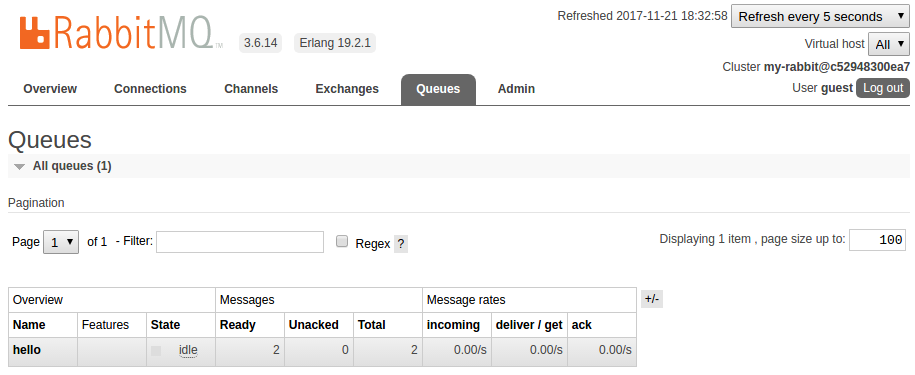
\includegraphics[width=\textwidth,keepaspectratio]{rabbit}
	\label{fig:rabbit}
\end{figure}

\subsection{Send and Receive Containers}
In order to \textit{dockerise} the messaging system images need to be built for the \textit{send} and \textit{receive} programs. In order to do this a Dockerfile is needed (Dockerfiles shown in appendices \ref{send-dockerfile} and \ref{receive-dockerfile}).
Dockerfiles contain commands and instructions for building an image. These include:
\begin{itemize}
	\item \textbf{Base Image:} A base image to use for the build e.g a Ubuntu image;
	\item \textbf{Instructions:} ~Steps necessary to configure the image such as a commands to install required software;
	\item \textbf{Arguments}: Arguments which may be needed for the instructions.
\end{itemize}
For the \textit{send} and \textit{receive} images, the Dockerfiles detail a base Python image, installs the required Pika software and adds the necessary python scripts to send or receive messages(scripts shown in appendices \ref{send-script} and \ref{receive-script}).

The IP address of the RabbitMQ container is also added as a build argument. This allows the scripts to communicate with the RabbitMQ container. In this case it means that the IP address for the messaging service is baked into the image. This may not be desirable as it does not as it does not allow flexibility such as scaling (adding more RabbitMQ containers if necessary). It will be shown later that service discovery can be used for this.

With the Dockerfiles created, the images are built using the following commands:
\begin{lstlisting}[language=bash]
docker build --build-arg rabbitmq_ip=$IP -t send:1 .
docker build --build-arg rabbitmq_ip=$IP -t receive:1 .
\end{lstlisting}

With the images built they are run as follows:
\begin{lstlisting}[language=bash]
docker run -ti send:1 /bin/bash
\end{lstlisting}
This runs the container and opens a terminal to it at which point the send program can be run:
\begin{lstlisting}[language=bash]
chmod +x /code/send.py
/code/send.py
\end{lstlisting}
Similarly for the \textit{receive} program:
\begin{lstlisting}[language=bash]
docker run -ti receive:1 /bin/bash
\end{lstlisting}
This runs the container and opens a terminal to it at which point the send program can be run:
\begin{lstlisting}[language=bash]
chmod +x /code/receive.py
/code/receive.py
\end{lstlisting}

Three containers are now running and messages can be passed as desired by running \textit{send.py} and \textit{receive.py}.

\begin{figure}[H]
	\setlength{\belowcaptionskip}{15pt plus 3pt minus 2pt}
	\caption{Containers Showing Message Passing}
	\centering
	%\includegraphics[width=\textwidth,height=\textheight,keepaspectratio]{diagram}
	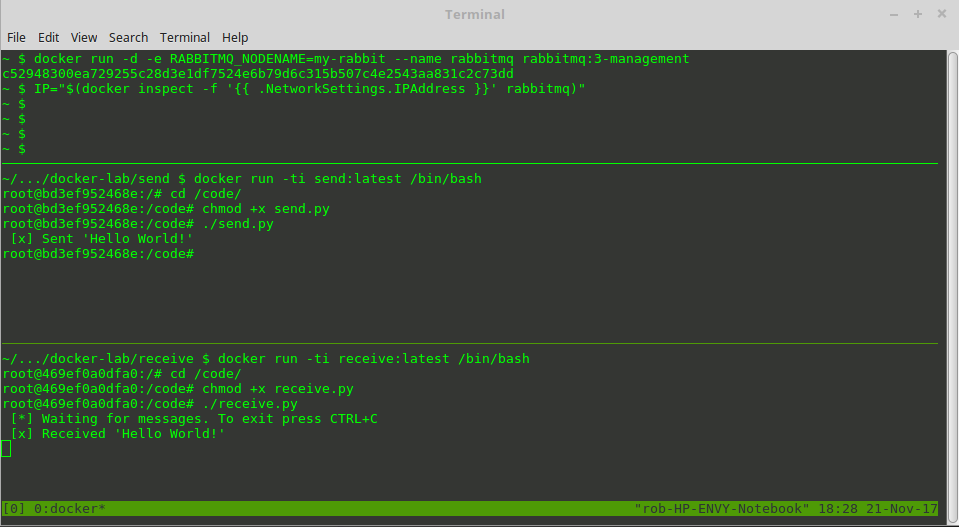
\includegraphics[width=\textwidth,keepaspectratio]{send-receive}
	\label{fig:rabbit}
\end{figure}